\section{Retrieving Images in Clusters}
\label{sec_introduction}

Many semantic image analysis algorithms, e.g. for image categorization or content detection, require training data on which the relevant features can be learned. Obtaining such training data can be a troublesome task, especially when the training set is created manually from scratch. If, for example, an algorithm shall be trained to identify and categorize kinds of food, one would have to think of all possible kinds of food, search for corresponding images and divide them into homogeneous groups. \\
A good place to search for images are online photo communities like Flickr\footnote{https://www.flickr.com/}, which provide vast amounts of collaboratively tagged images. These communities are also called folksonomies\index{Folksonomy}, i.e. socially indexed collections.
Although folksonomies can be good sources for training data due to the semantic metadata that tags provide, several problems exist: First of all, annotations are often of poor quality, since anyone can tag anything with no existing control mechanisms. Secondly, one can only search for a specific term, and will obtain images for all of the term's meanings. However, this way the retrieval is limited to only those images which are annotated with the exact term as a tag. This results in the fact, that usually no semantic relations to other terms are provided. Furthermore, the images will be of a very large visual diversity, which is often not desired. \\

This work presents a tool whose main aim is to create homogeneous groups of semantically and visually similar pictures for a given topic in order to aid with the laborious assembly of training and test data sets. The main challenges encountered were homonymy\index{Homonymy} of keywords (the fact that one word can have multiple meanings), low quality of tags and other annotations, and the consideration of both semantic and visual information about a picture.

\subsection{Clustered Tree Nodes Approach}
The tool has been implemented as a Python web application, using WordNet\footnote{http://wordnet.princeton.edu/} for semantic image analysis, SimpleCV\footnote{http://www.simplecv.org/} for visual image analysis and Flask\footnote{http://flask.pocoo.org/} together with Bootstrap\footnote{http://getbootstrap.com/} for the frontend presentation.\\
It provides ready-to-use semantically and visually homogeneous image clusters for a given topic, or search term. This is achieved by 2 major phases: First, spanning a tree of subordinate terms of the topic and retrieving related images by their keywords for each node of the tree. Second, clustering the images by their predominant keywords as well as by colors and edge structure. The following figure \ref{fig_overallprocess} illustrates these two main phases of the tool.

\begin{figure}[h]
\centering
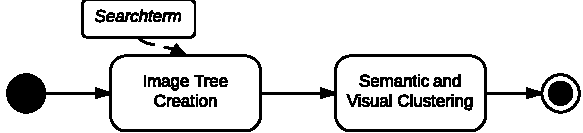
\includegraphics[]{images/search_process_highlevel.pdf}
\caption{The two main phases of the clustered image search}
\label{fig_overallprocess}
\end{figure}

\subsection{Web Interface}

\begin{figure}[!htb]
  \minipage{0.49\textwidth}
    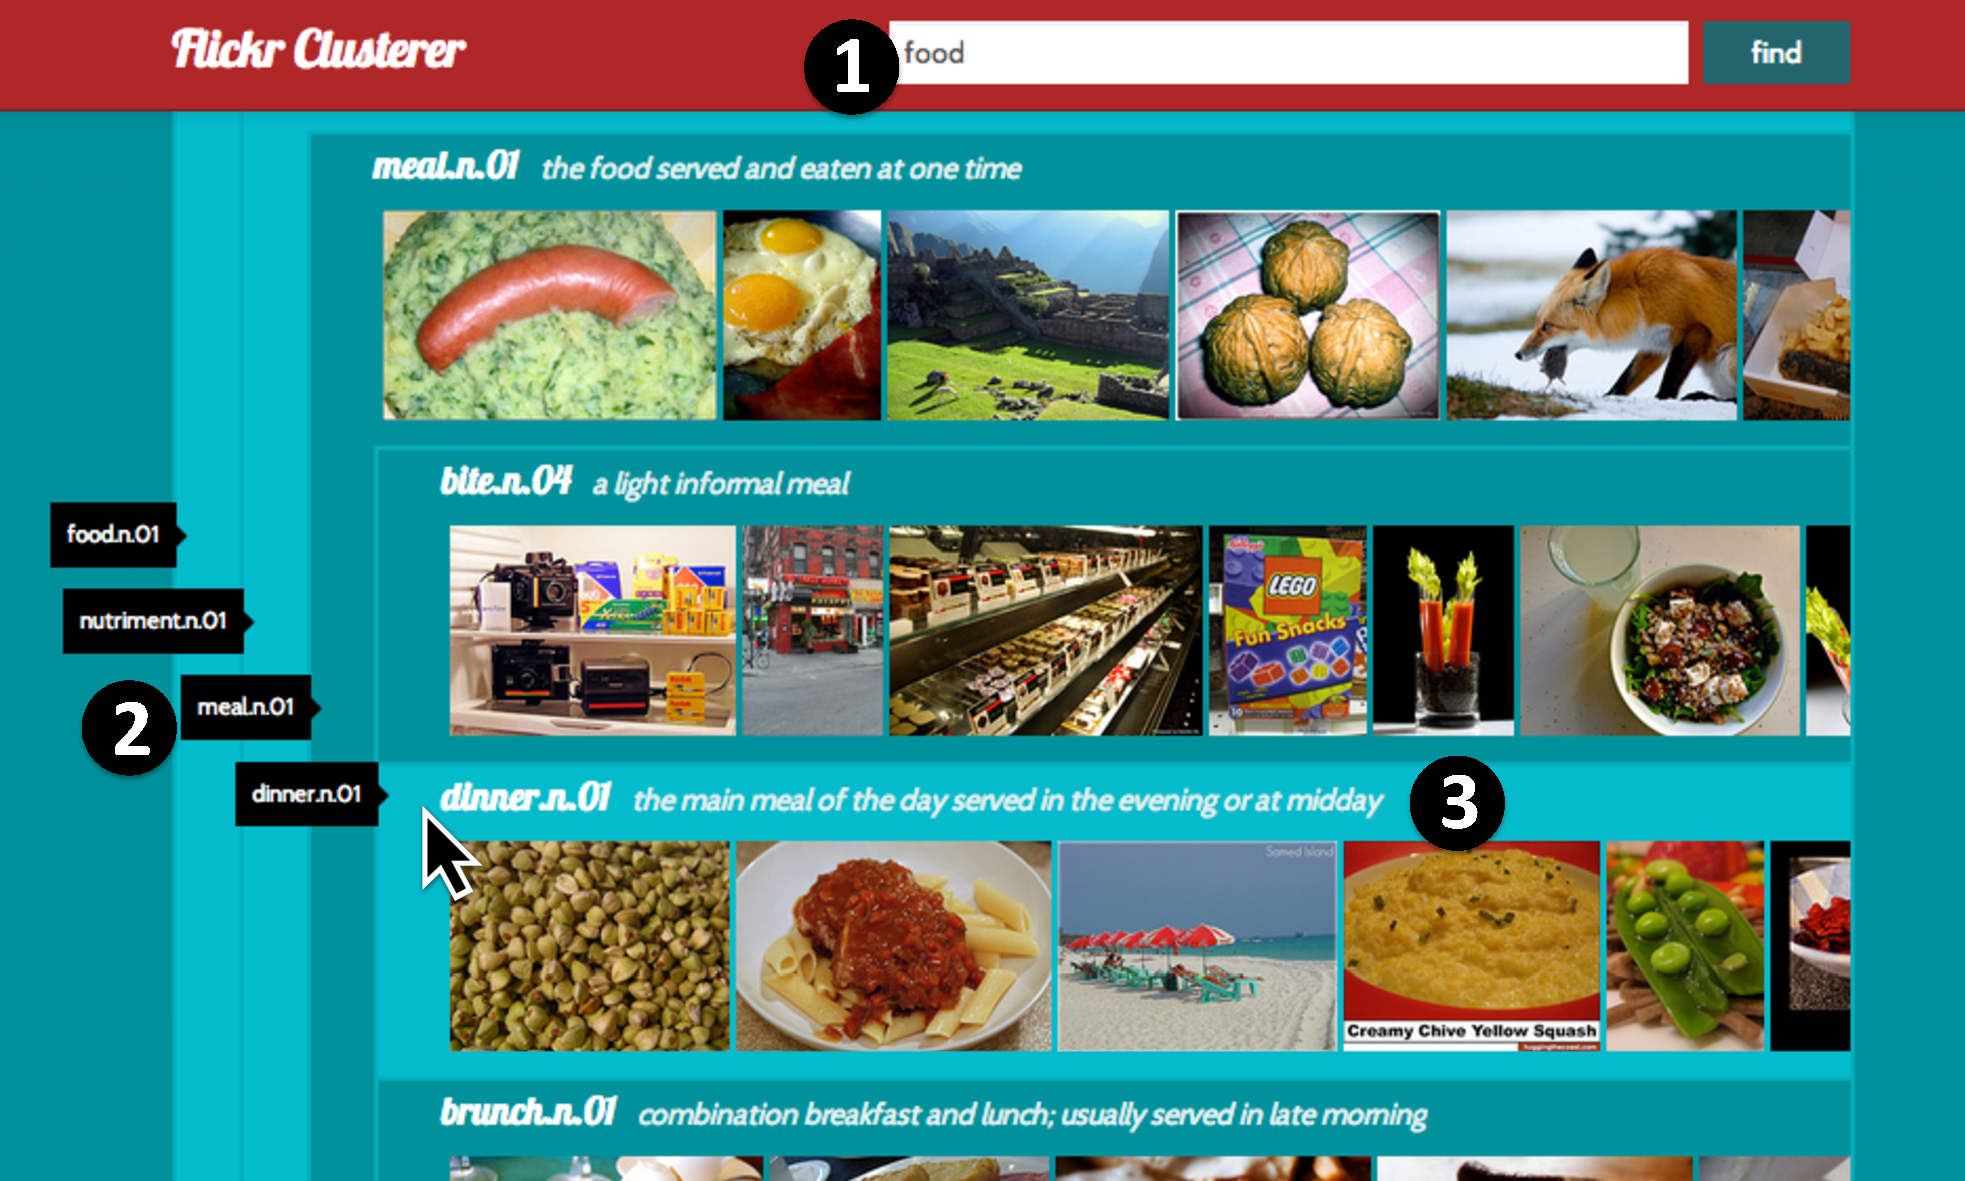
\includegraphics[width=\linewidth]{images/webfrontend-screenshot_1.pdf}
    \caption{Overview of the web interface (1) search term entered by user (2) semantic hierarchy (3) each line represents one hyponym of the entered search term with associated images}\label{fig_webinerface_1}
  \endminipage\hfill
  \minipage{0.49\textwidth}
    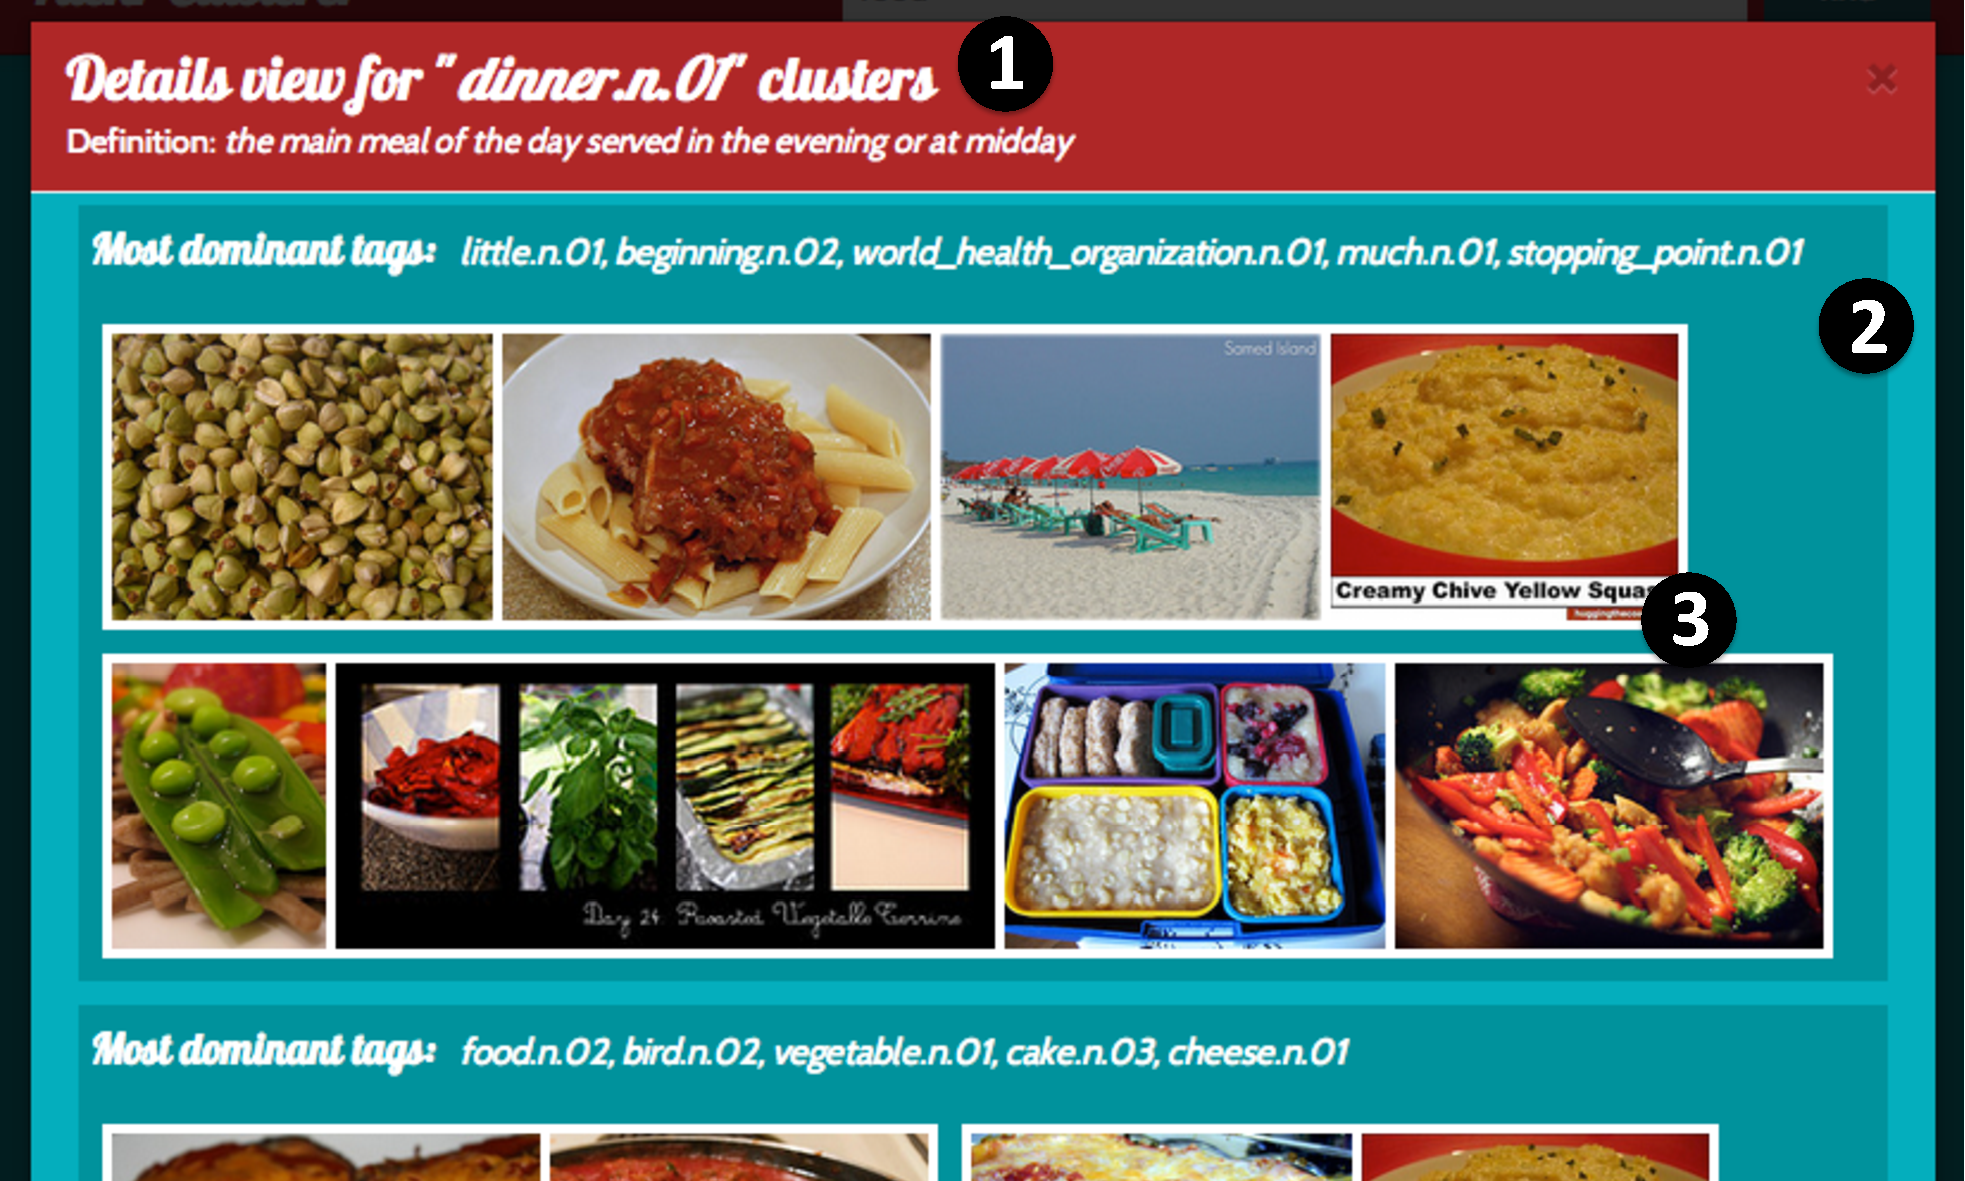
\includegraphics[width=\linewidth]{images/webfrontend-screenshot_2.pdf}
    \caption{Details view for one hyponym (1) selected hyponym with definition (2) dark cyan background groups different semantic clusters (3) white background groups visual clusters}\label{fig_webinerface_2}
  \endminipage\hfill
\end{figure}

\todo{In progress: Screenshot and explanation of our tool (What does it show?)}

After users entered a search term on the web interface (figure \ref{fig_webinerface_1}.1), they will be presented with a result tree. 
Each meaning WordNet finds for the given search term will result in a root node. 
Hyponyms of each node will then be rendered as sub nodes. 
This continues, until no more hyponyms can be found. 
As figure \ref{fig_webinerface_1}.2 shows, this hierarchy can then also be seen when hovering over the image rows.
For each row, the users now see a preview of the images found for this particular meaning of their search term (\ref{fig_webinerface_1}.3).

If one search term now strikes the user's attention, they can get detailed information by clicking on the images. 
Figure \ref{fig_webinerface_2} shows the \emph{details view}, where the definition of the particular hyponym can be found (\ref{fig_webinerface_2}.1). 
In the details view, the images now appear in more fine grained clusters.
The dark cyan background groups semantically similar images (\ref{fig_webinerface_2}.2) which have many other tags in common. These most dominant tags are also shown for each semantic sub cluster.
Within the semantic clusters, the white containers group visually similar images (\ref{fig_webinerface_2}.3). It is in these containers that users can find visually similar images belonging to one semantic topic of the given search term.

\bigskip

After giving an overview of Related Work in chapter 2, we present how we analyze the image annotations and the user's search term to retrieve relevant images in chapter 3. The methods applied to cluster the images semantically and visually are described in chapter 4. Chapter 5 explains how we evaluate our approach, while the evaluation results are discussed in chapter 6. At last, chapter 7 gives ideas for improvement and possible future work.
